\documentclass[a4paper, 11pt]{report}
\usepackage[utf8]{inputenc}
\usepackage[T1]{fontenc}
\usepackage{lmodern}
\usepackage{fancyhdr}
\usepackage{epstopdf}
\usepackage{graphicx}
\usepackage{caption}
\usepackage{hyperref}
\usepackage{url}
\usepackage{eurosym}
\usepackage{titlepic}
\usepackage[french]{babel}
\usepackage[top=2cm, right=2cm, bottom=2cm, left=2cm]{geometry}
\usepackage{graphicx}
\usepackage[T1]{fontenc}


\title{REX Minotaure}


\date{2019}

\titlepic{
\includegraphics[width=0.7\textwidth]{images/LogoMinotaure.png}}

\begin{document}

\maketitle

\tableofcontents

\part{Introduction}

Ce REX a pour rôle d'accumuler les connaissances de générations en générations. Souvent, la coupe de france de robotique demandera l'utilisation d'outils spéciaux comme des ventouses mais celles-ci ne seront pas utilisées les années suivantes et les connaissances dessus seront ainsi perdues.

Dès que vous rencontrez quelque chose qui n'est pas dans ce REX, que vous voulez faire part d'une expérience enrichissante, d'une astuce ou d'un problème récurrent, il ne faut hésiter à l'ajouter à ce REX (Objectif: il faut que ce REX soit plus épais que le poly de MMC).

Minotaure ne pourra s'améliorer que si on accumule l'expérience au fur et à mesure des années (chose difficile avec les césures).

\section{Histoire}
Minotaure existe depuis 2004. C'est un P03 qui a créé l'association pour pouvoir continuer à participer à la coupe de france de robotique hors de la mécatronique (il a d'ailleurs créé sa propre entrerprise qui sponsorise des équipes de la coupe de france de robotique).

\section{Rôle de Minotaure}

\section{Les différentes équipes au cours du temps}

\subsection{2017-2018}

\subsection{2018-2019}

\part{Composants}

\chapter{Actionneurs}

\section{Moteurs pas-à-pas}

\begin{figure}[h]
\begin{centering}
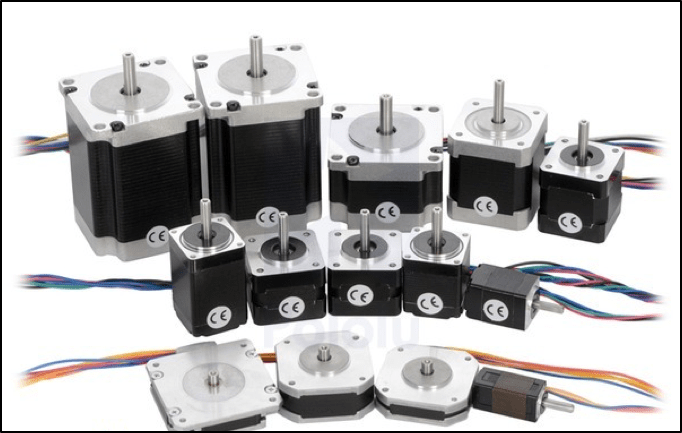
\includegraphics[width=0.7\textwidth]{images/MoteurPasAPas.png}
\caption{Moteur pas-à-pas}
\par\end{centering}
\end{figure}

Les moteurs pas-à-pas sont des moteurs électriques brushless à courant continu. Il en existe 3 types:
\begin{description}
\item[Moteurs pas-à-pas à aimants permanents] Un aimant permanent est solidaire de l'axe du moteur (rotor). Des bobines excitatrices sont placées sur la paroi du moteur (stator) et sont alimentées chronologiquement. Le rotor s'oriente suivant le champ magnétique créé par les bobines.
\item[Moteurs pas-à-pas à reluctance variable] Il s'agit d'un moteur qui comporte un rotor à encoches se positionnant dans la direction de la plus faible réluctance. Ce rotor, en fer doux, comporte moins de dents qu'il n'y a de pôles au stator.
\item[Moteurs pas-à-pas hybrides synchrones]Ils combinent les 2 technologies précédentes, et sont pluschers. Leur intérêt réside dans un meilleur couple, une vitesse plus élevée.
\end{description}

\begin{figure}[h]
\begin{centering}
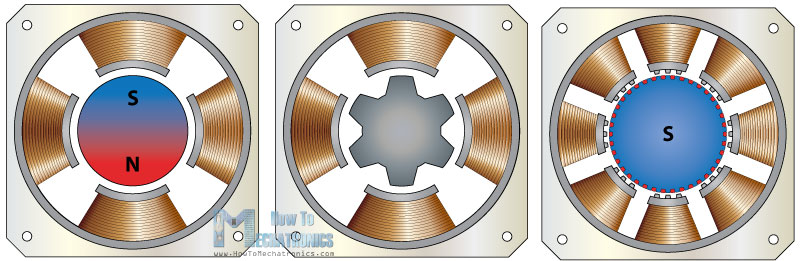
\includegraphics[width=0.7\textwidth]{images/DifferentsMPP.jpg}
\caption{De gauche à droite: Aiment permanent, Reluctance Variable, Hybride}
\par\end{centering}
\end{figure}

Le nombre de phase d'un moteur correspond au nombre de bobines indépendantes. Ce nombre est proportionnel à la précision du moteur.
Parmi les moteurs pas-à-pas à 2 phases, il existe 2 sous-groupes:
\begin{description}
\item[Unipolaire:]Les plus simples d'utilisation et moins chers. Leur connecteur est constitué de 6 fils. Chaque pôle est constituée de deux bobines enroulées en sens inverse sur les pôles du stator. Pour changer le sens du champ magnétique dans un pôle, il faut alimenter l'une ou l'autre de ces deux bobines. Le sens du courant est constant.
\item[Bipolaire:]Les plus puissants. Leur connecteur est constitué de 4 fils. Chaque pôle du stator est constitué d'une seule bobine, et nécessite donc deux fils d'alimentation. Le sens du courant change tout le temps.
\end{description}

Les moteur les plus courants sont ceusx à aimants permanents et les hybrides.

Vidéos explicatives des moteurs pas-à-pas hybrides: \url{https://www.youtube.com/watch?v=eyqwLiowZiU}

\textbf{Utilisation:} Imprimantes (3D ou simple), photocopieurs, robotique, pousse-seringue,...

\textbf{Avantages:}
\begin{itemize}
\item Contrôle en position possible donc en vitesse sans avoir besoin d'une boucle fermée
\item Précision
\item Existence d'un couple d'arrêt
\end{itemize}

\textbf{Inconveinients:}
\begin{itemize}
\item Le couple maximal est inversement proportionnel à la vitesse maximal, c'est-à-dire qu'un moteur pas-à-pas sera capable de fournir le plus de couple pour de faible vitesse de rotation.
\item Lent, ils ne dépassent pas les 3000 tr/min en général.
\item Volumineux et lourd
\item Fonctionnement plus complexe qu'un moteur à courant continu
\item Résonance du moteur
\end{itemize}

\textbf{Précautions:}
\begin{itemize}
\item Le bobinage des moteurs pas-à-pas est très fragile. Si les cables sont mals branchés, il peut y avoir un court-circuit entre les 2 bobinages ce qui "cassera" le moteur pas-à-pas. Il faut utiliser un ohmmètre pour distinguer les fils. 2 fils reliés à la même bobine auront une résistance tandis que d'autres connections afficheront soit rien soit une très grande résistance.
\item Toujours manipuler les fils quand il n'y a pas de courant. Un court-circuit peut facilement détruire les moteurs.
\end{itemize}

Pour distinguer les différents moteurs pas-à-pas, la norme NEMA est utilisée. Cette norme indique la taille du moteur et donc sa puissance. Le nombre représente la surface de la face de l'axe du moteur en pouce carré. Ainsi, un moteur NEMA 11 aura une face d'une surface de 1,1 pouces carrés.

Le couple du moteur est proportionnel au courant.

Une bonne documentation fournira la vitesse et la puissance d'un moteur pas-à-pas. Cependant, il se peut que cela ne soit pas le cas. Dans ce genre de situation, il est possible de calculer des indicateurs sur la vitesse:

\begin{figure}[h]
\caption{Calcul de la vitesse d'un moteur pas-à-pas}

\begin{centering}
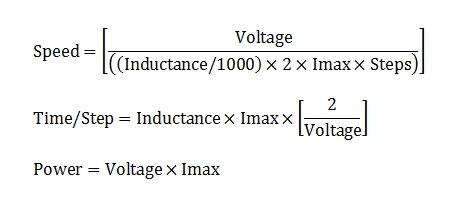
\includegraphics[width=0.7\textwidth]{images/SpeedCalculator.jpeg}
\par\end{centering}
\end{figure}

Une version en ligne permet de faire le calcul directement.
\url{https://www.daycounter.com/Calculators/Stepper-Motor-Calculator.phtml}

\textbf{Fournisseurs:} Stepper Online, Gotronic,...

\begin{figure}
\begin{centering}
\caption{Gauche: Graphique du couple de maintien en fonction du courant consommé - Droite: Réponse en angle à un échelon}
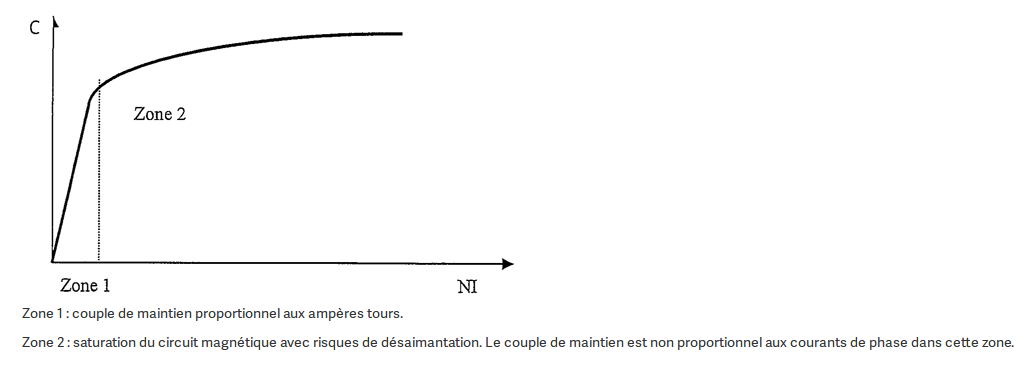
\includegraphics[width=0.7\textwidth]{images/CoupleMaintien.png}
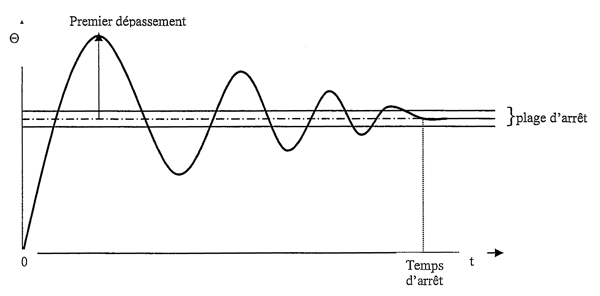
\includegraphics[width=0.7\textwidth]{images/reponse_indicielleMPP.png}
\par\end{centering}
\end{figure}

Pour plus d'information techniques, regarder: \url{https://www.mdp.fr/documentation/lexique/pas-a-pas/notions-techniques.html}

\subsection{Utilisation}

Ce site donne une bonne présentation des moteurs pas-à-pas et comment les utiliser: \url{https://eskimon.fr/tuto-arduino-603-a-petits-pas-le-moteur-pas-\%C3\%A0-pas#se-servir-du-moteur}

Sinon, le contrôleur de moteurs pas-à-pas utlisé pour l'édition 2019 était celui-ci:

\url{https://fr.rs-online.com/web/p/kits-de-developpement-pour-commande-de-moteur/1646982}

Un driver en C a été écrit par Matthieu Vignes et est disponible sur le Git.

\section{Moteurs à courant continu}

Les moteurs à courant continu sont les plus courants. Ils ne sont cependant utilisés que dans des cas basiques.

\begin{figure}[h]
\begin{centering}
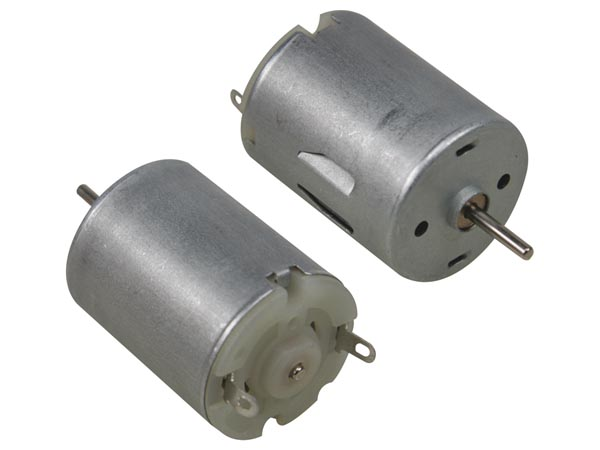
\includegraphics[width=0.7\textwidth]{images/MoteurDC.jpeg}
\caption{Moteurs à courant continu}
\par\end{centering}
\end{figure}

\textbf{Avantages:}
\begin{itemize}
\item Très simple d'utilisation
\item Taille faible pour un couple puissant
\end{itemize}

\textbf{Inconvénients:}
\begin{itemize}
\item La loi entre la tension aux bornes du moteur et la vitesse de rotation ne sera pas la même pour des modèles identiques de moteur.
\item Aucun retour d'information et contrôle en position ou en vitesse impossible en boucle ouverte.
\end{itemize}


\subsection{Utilisation}
Pour un moteur à courant continu, la vitesse de rotation est propotionnelle à la tensionà ses bornes. Cependant, étant donné qu'il est difficile de générer une tension variable, le moteur DC est le plus souvent alimenté à travers un hacher avec une tension fixe.
\url{https://wiki.mchobby.be/index.php?title=Pont-H_L298N}

Le pont L298N est la meilleure méthode pour contrôler des moteurs à courant continu.

Il est aussi possible de de choisir la tension à fournir pour contrôler le moteur avec des transistors:
\url{https://openclassrooms.com/fr/courses/2778161-programmez-vos-premiers-montages-avec-arduino/3285333-le-moteur-a-courant-continu-partie-1-transistors-et-sorties-pwm}

\section{Moteurs brushless}
Les moteurs brushless comme leur nom l'indique sont des moteurs à courant continu sans balais. De ce fait, ils s'usent moints rapidement que les moteurs. Ils sont notament utilisés en aéromodélisme pour leur endurance et la puissance qu'ils peuvent délivrer. A la place des balais, 3 cables d'alimentations sont nécessaires pour les phases des différentes bobines (alimentation triphasée).

Pour inverser le sens de rotation d'un moteur brushless, il suffit d'inverser la connection de 2 de ses 3 cables.

\begin{figure}[h]
\begin{centering}
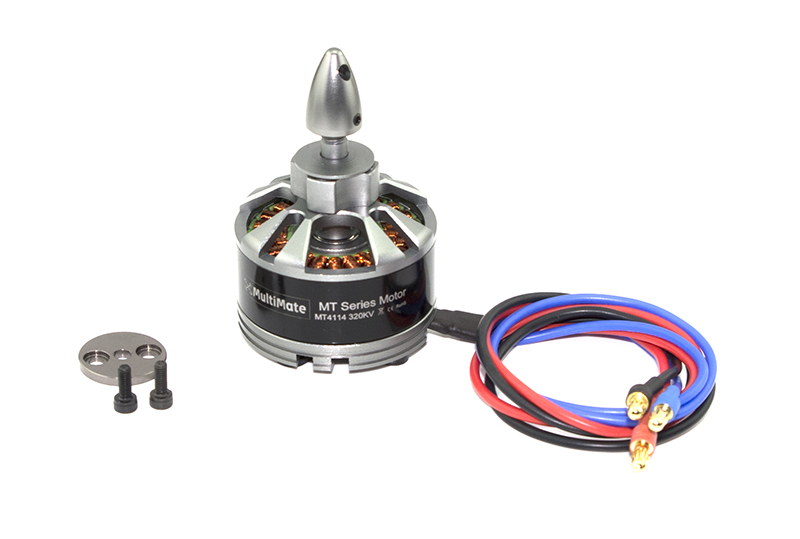
\includegraphics[width=0.7\textwidth]{images/MoteurBrushless.jpg}
\caption{Moteur brushless}
\par\end{centering}
\end{figure}

Avantages:
\begin{itemize}
\item Vitesse asservie
\item Fabriqué pour tourné à de grandes vitesses
\end{itemize}

Inconvénients:
\begin{itemize}
\item Nécessité d'un ESC
\end{itemize}

\subsection{Utilisation}
Pour utiliser un moteur brushless, il est nécessaire d'utiliser un  ESC (Electronic Speed Controller) 

\begin{figure}[h]
\begin{centering}
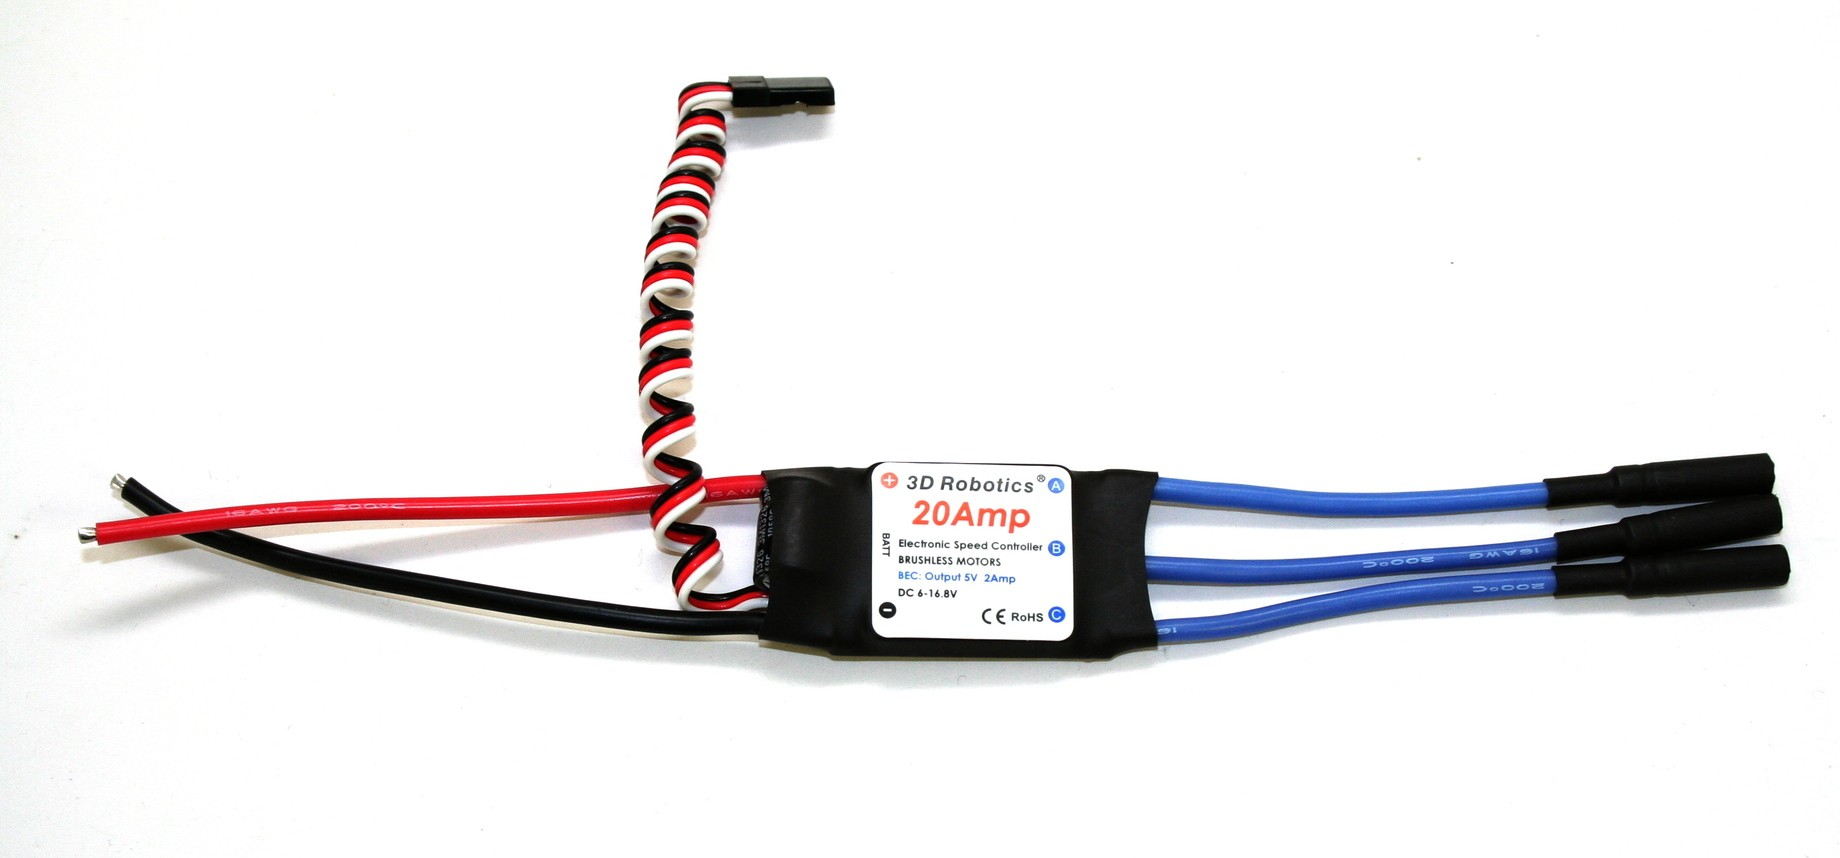
\includegraphics[width=0.7\textwidth]{images/ESC.jpg}
\caption{ESC}
\par\end{centering}
\end{figure}

\section{Servomoteurs}

\begin{figure}[h]
\begin{centering}
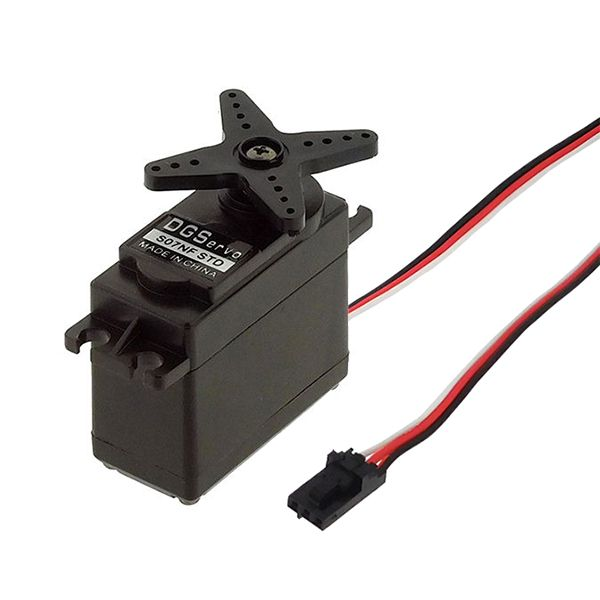
\includegraphics[width=0.7\textwidth]{images/servomoteur.jpg}
\caption{Servomoteurs}
\par\end{centering}
\end{figure}

C'est un moteur à courant continu asservi. Il est souvent utiliser pour effectuer de petits mouvements. On le commande en angle et il maintient ensuite sa position peut importe l'effort exercé dessus (bien sûr il casse si on force trop).

\begin{figure}[h]
\begin{centering}
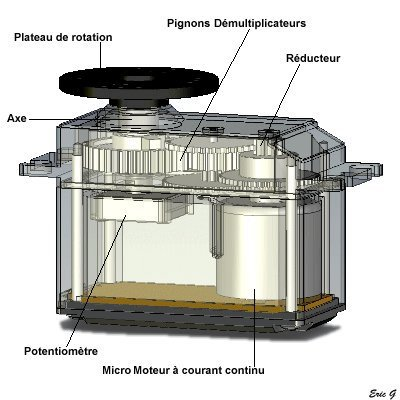
\includegraphics[width=0.5\textwidth]{images/schemaServo.jpg}
\caption{Schéma d'un servomoteur}
\par\end{centering}
\end{figure}

Il est composé d'un moteur à courant continu, d'une réducteur, d'un potentiomètre et d'un circuit intégré. C'est le potentiomètre qui fournit le retour en angle (d'où l'impossibilté de positioner de manière absolue sur plus de 180\degre)

\textbf{Avantages:}
\begin{itemize}
\item Simple d'utilisation
\item Contrôle en position
\end{itemize}

\textbf{Inconveignients:}
\begin{itemize}
\item Aucun retour sur la position
\item Limité à 160-180 \degre de rotation (Il existe cependant des servos à rotation continu)
\end{itemize}

\subsection{Utilisation}

\subsubsection{Cablage}

Image des différents cables

Il faut 3 cables pour utiliser un servomoteur:
\begin{itemize}
\item Masse
\item V+ : cela dépend des servomoteirs mais ce sera en général 5V
\item Signal: un signal PWM est utilisé pour commander 
\end{itemize}

\subsubsection{Signaux PWM}

\begin{figure}[h]
\begin{centering}
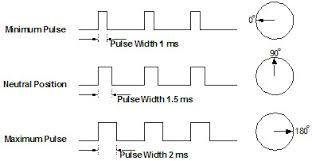
\includegraphics[width=0.5\textwidth]{images/PWMservo.jpeg}
\caption{Signal PWM pour contrôler un servomoteur}
\par\end{centering}
\end{figure}

La durée d'un signal PWM (Pulse Width Modulation) est proportionnelle à la commande. En général, la fréquence est de 50 Hz pour les servomoteurs mais elle peut être différente pour d'autres applications.

\section{Les Dynamixels}
Ce sont les actionneurs le plus souvent utilisé en robotique. Ils sont produits exclusivement par la société Robotis.

Avantages:
\begin{itemize}
\item Retour de beaucoup d'informations: courant consommé, couple appliqué, vitesse et position,...
\item Configurable
\end{itemize}

Inconvénients:
\begin{itemize}
\item Très difficile d'utilisation. Il faut utiliser un connecteur spécial et coûteux pour les débuguer.
\item Plus fragiles que les servomoteurs.
\end{itemize} 

\chapter{Système pneumatique}

\section{Pompe}

\subsection{Pneumatique}

\subsection{Hydrolique}

On peut ne pas pouvoir inverser le sens

\section{Ventouse}
Les ventouses sont très utilses pour se saisir d'objets ayant des surfaces relativement plane et lisse.

Ventouse avec et sans souflet

Avantage:

Inconveignents:

Fournisseur: RS

\section{Accessoires et autres}

\chapter{Communication}

\section{Radio}

\begin{figure}[h]
\begin{centering}
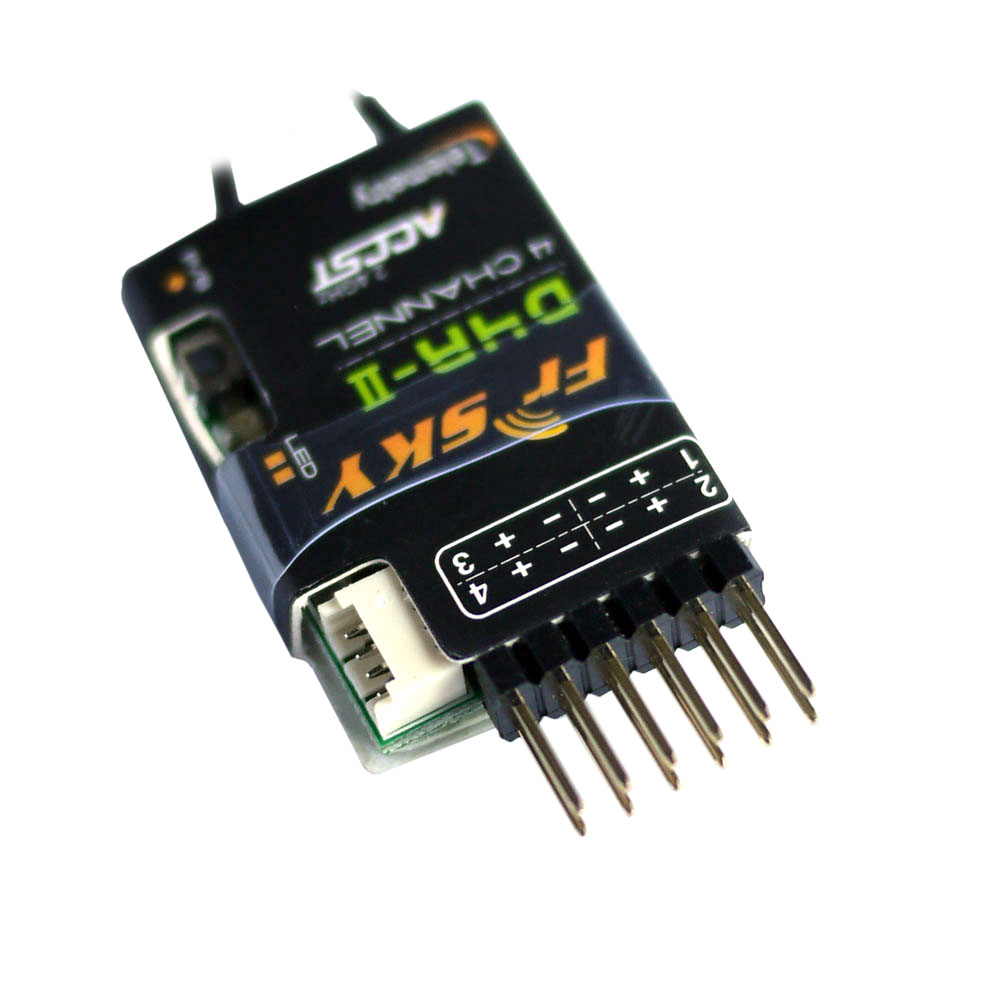
\includegraphics[width=0.5\textwidth]{images/recepteurRadio.jpg}
\caption{Récepteur radio}
\par\end{centering}
\end{figure}

En modélisme, des radiocommandes sont utilisées pour commander avion, bateau ou voiture. De nos jours, la fréquence utilisée en majorité est la 2.4GHz car plusieurs personnes peuvent utiliser cette fréquence sans risquer d'interférences mais avant, des fréquences de l'ordre du MHz étaient utilisées. Ces fréquences dépendent du pays mais en France, on pouvait utiliser 42Mhz et 58Mhz. Ces fréquences ont l'avantage d'avoir une plus grande portée.

\begin{figure}[h]
\begin{centering}
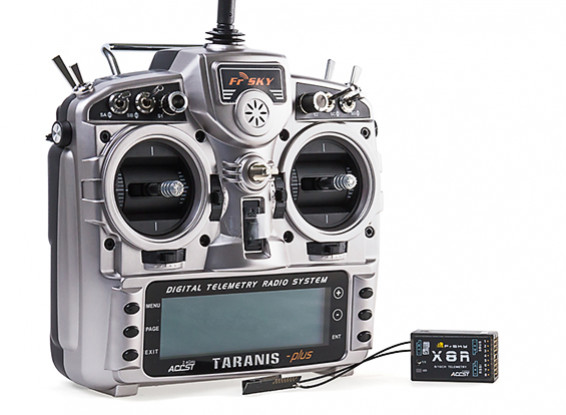
\includegraphics[width=0.5\textwidth]{images/taranis.jpg}
\caption{Radiocommande}
\par\end{centering}
\end{figure}

\section{Bluetooth}

\begin{figure}[h]
\begin{centering}
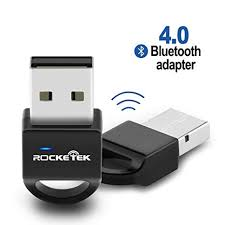
\includegraphics[width=0.5\textwidth]{images/dongleBluetooth.jpeg}
\caption{Adaptateur bluetooth}
\par\end{centering}
\end{figure}

On peut utiliser le Bluetooth pour faire communiquer deux appareils à courte distance. C'est en général ce qui est fait pour transmettre des informations entre 2 Raspberry Pi.

Le Bluetooth utilise 2.4GHz comme le Wifi mais il n'est pas utilisé pour les mêmes applications. Il permet un débit de données plus faibles et à une plus faible portée. En contrepartie, le Bluetooth consomme moins de courant que le Wifi. Les protocoles de communication ne sont aussi pas les mêmes, tout comme les organismes qui gèrent les normes pour le Bluetooth et le Wifi.

\section{Module Xbee}

\begin{figure}[h]
\begin{centering}
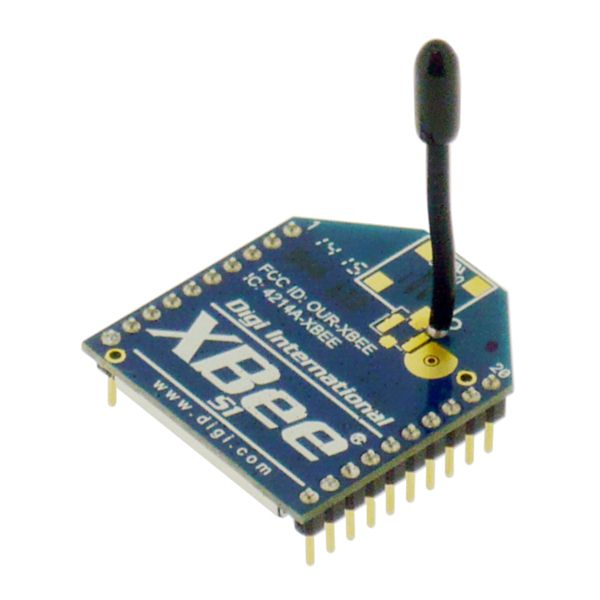
\includegraphics[width=0.5\textwidth]{images/XBee.jpg}
\caption{Module XBee}
\par\end{centering}
\end{figure}

XBee est une marque qui produit des interfaces réseaux. Il en existe une grande diversité. On peut les distinguer par leur architecture réseau, la fréquence utilisée, le type d'antenne et la porté/puissance du signal.

\subsection{Architecture réseau}
Différentes architectures réseaux ont été dévelopées pour les modules Xbee en fonction des besoins.
\subsubsection{•}

\subsubsection{•}

\chapter{Cartes électroniques}

\section{Arduino}

\begin{figure}[h]
\begin{centering}
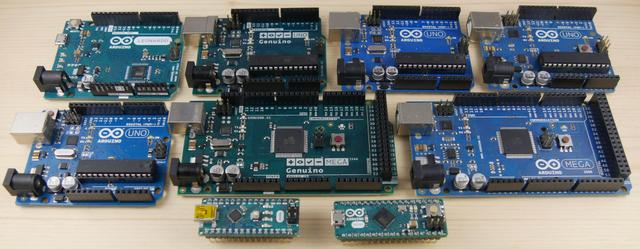
\includegraphics[width=0.5\textwidth]{images/cartesArduino.jpg}
\caption{Différentes cartes Arduino}
\par\end{centering}
\end{figure}

Les cartes Arduino sont les cartes de prototypage les plus populaires de part leur simplicité d'utilisation et leur rapport qualité-prix. La plus répandue est la carte Arduino Uno.

\section{Raspberry Pi}
C'est un micro-ordinateur. Elle est donc beaucoup plus puissante que la Teensy ou les cartes Arduino. Cependant, elle est aussi limité dans ses capacités.

Avantages:
\begin{itemize}
\item Ports USB
\item Wifi et bluetooth intégrés pour la version 3B+
\item Plus de puissance de calcul
\item Possibilités de programmer dans n'importe quel language.
\end{itemize}

Inconvénients:
\begin{itemize}
\item Il est difficile de générer des signals PWM
\item Seulement une vrai liaison série disponible et encore. Elle est normalement dédiée au bluetooth mais on peut l'utiliser pour autre chose si on utilise pas le Bluetooth. Il y a aussi une autre pseudo liaison série mais elle est très limitée.
\end{itemize}

\subsection{Ports USB}

\subsubsection{Interface série}

\subsubsection{Courant}

\section{Teensy}
La teensy est en résumé une version miniature d'une carte arduino, en plus puissante. Elle possède notament plus de sortie série. Elle se programme exactement de la même manière qu'une carte arduino.

\section{Shield}
Les différentes cartes électroniques ne possèdent pas tous les capteurs ou sorties nécessaires pour un projet. Pour compenser ces problèmes, des Shield ont été créés. Ce sont des extensions des cartes électroniques très faciles d'utilisation. Cela coûte bien sûr moins cher de les faire soit même mais on est certain au moins que c'est fiable avec un shield.

Différents shields:
\begin{itemize}
\item GNSS
\item Servo
\end{itemize}

\chapter{Capteurs}

\section{GNSS}
GNSS (Global Navigation Satellite System)  designe un ensemble de composants reposant sur une constellation de satellites artificiels permettant de fournir à un utilisateur par l’intermédiaire d'un récepteur portable de petite taille sa position 3D, sa vitesse et l'heure.

Il est important de distinguer GPS et GNSS. GPS (Global Positionning System) correspond à la constellation de satellites des Etats-Unis qui appliquent le principe de GNSS. C'est un abus de language.

\textbf{Avantages:}
\begin{itemize}
\item Position absolue
\item Donne aussi la vitesse du véhicule (dans)
\end{itemize}

\textbf{Inconvénients:}
\begin{itemize}
\item La précision des mesures dépend fortement de la qualité du signal. En milieu urbain, les immeubles bloquent certains satellites et peuvent générer des multipaths.
\end{itemize}

\textbf{Fournisseurs:} Ublox, Emlid,...

Il existe différents modes de positionnement par GNSS aujourd'hui dont certains peuvent donner une  précision allant jusqu'au centimètre.

\subsection{NMEA}

\subsection{Mode de positionnement}

\subsubsection{Single}

\subsubsection{PPP}

\subsubsection{Différentiel}


\section{LIDAR}

\begin{figure}[h]
\begin{centering}
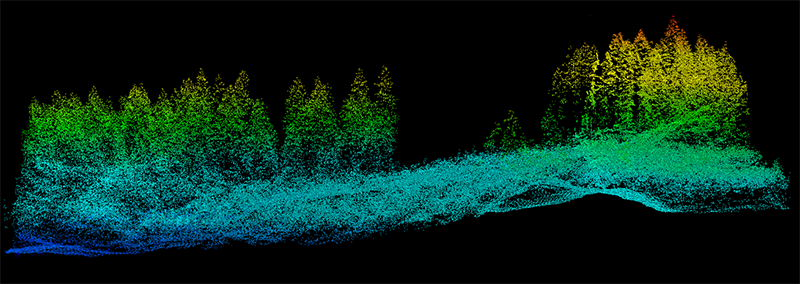
\includegraphics[width=0.5\textwidth]{images/NuageDePoints.png}
\caption{LIDAR de SLAMTEC}
\par\end{centering}
\end{figure}

Acronyme pour Light Detection And Ranging, ce capteur permet de générer un nuage de point de l'environnement qui l'entoure. Le LIDAR fait cela grâce à un laser qui mesure la distance avec un obstacle. Contrairement à un capteur infrarouge actif, le laser du LIDAR est très directif et permet des mesures plus précises. En connaissant la configuration du LIDAR, on connaît la direction du laser et donc la direction de l'obstacle. Les LIDARs que nous utilisons sont font juste des mesures dans un plan mais il existe des LIDARs qui fournissent des nuages de points en 3D.

\begin{figure}[h]
\begin{centering}
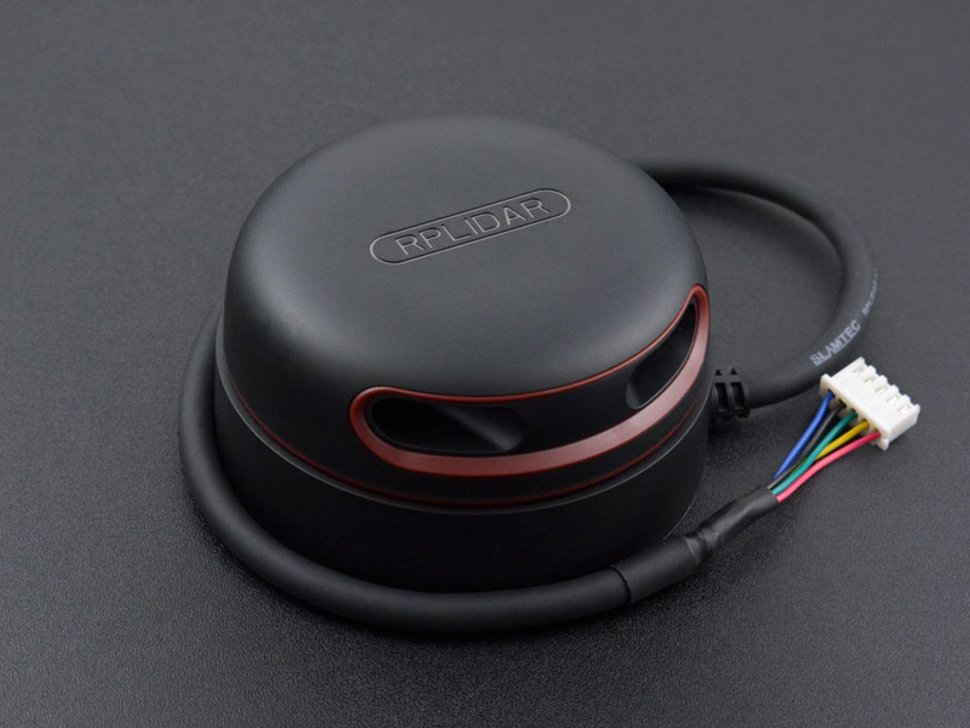
\includegraphics[width=0.5\textwidth]{images/RPLidar.jpg}
\par\end{centering}
\end{figure}

\subsection{Matériel}
\begin{description}
\item[Modèle:] A2M8
\item[Quantité:]2
\item[Fabricant:]Slamtech
\item[Fournisseur:]Robotshop
\end{description}


\subsection{Utilisation}
\begin{description}
\item[Positionnement:]En utilisant des techniques de SLAM, il est possible d'utiliser des balises posées sur le bord du terrain pour obtenir la position et l'orientation du robot. Le problème est que la résolution des LIDAR que Minotaure possède n'est pas suffisante pour détecter les balises partout sur le terrain.
\item[Détection d'obstacles:] Il est possible de détecter les robots adverses à partir du nuage de points. Pour cela, il faudrait faire une détection de blobs, qui correspondraient aux robots.
\end{description}

\section{Ultrason}

\section{Infrarouge}

\begin{figure}[h]
\begin{centering}
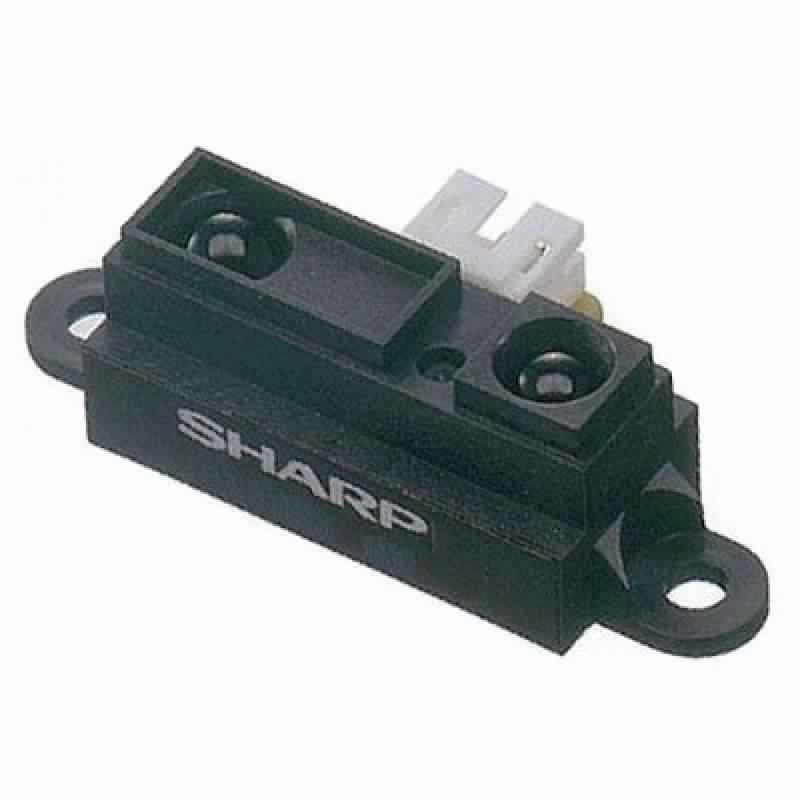
\includegraphics[width=0.5\textwidth]{images/capteurInfrarougeActif.jpg}
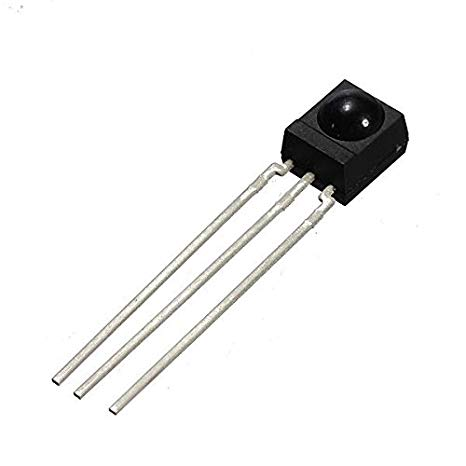
\includegraphics[width=0.5\textwidth]{images/capteurInfrarougePassif.jpg}
\caption{Capteurs infrarouges Actif (gauche) et passif (droite)}
\par\end{centering}
\end{figure}

On distingue 2 types de capteurs infrarouges, les capteurs passifs qui mesurent juste la lumière ambiante et les capteurs actifs qui génèrent aussi des ondes infrarouges. On pourrait aussi parler des caméras infrarouges, mais ce sont simplement des caméras qui mesurent captent les infrarouges en plus des ondes du domaine visible.

\textbf{Avantages:}
\begin{itemize}
\item Peu cher
\item Simple à mettre en oeuvre
\end{itemize}

\textbf{Inconvénients:}
\begin{itemize}
\item Très sensible à la lumière ambiante, les écalairages traditionnels émettent aussi des infrarouges qui peuvent induire le capteur en erreur.
\end{itemize}

\subsection{Utilisation}
Le capteur infrarouge actif est en général utilisé en tant que capteur d'obstacle. En fonction de la quantité d'ondes infrarouges reçues, on peut estimer la distance de l'obstacle. Le problème est que cette quantité varie en fonction de l'écalirage de l'environnement (notamment avec des projecteurs). Pour compenser ce problème, il est nécessaire de calibrer les capteurs infrarouges à chaque lancement.

La phase de calibration peut consister définissant le taux moyen d'infrarouge dans l'environnement en mesurant sur une certaine période ou en redéfinissant la valeur limite.

\section{Capteurs de fin de course}
Comme son nom l'indique, le capteur de fin de course permet d'observer les contacts. Ils sont aussi appelés interrupteurs ou détecteurs de position. Ce sont en soit des interrupteurs poussoirs avec des 


\section{Codeurs incrémentaux}

\begin{figure}[h]
\begin{centering}
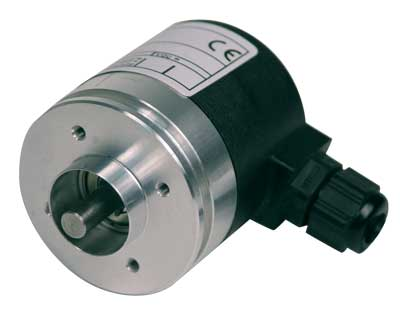
\includegraphics[width=0.5\textwidth]{images/photoCodeurIncremental.JPG}
\caption{Codeur Incrémental}
\par\end{centering}
\end{figure}

Les capteurs incrémentaux mesurent une rotation.

Il existe des codeurs incrémentaux absolus et relatifs. Cependant, les codeurs absolus sont très chers. En effet, chaque position doit avoir sa m

\begin{figure}[h]
\begin{centering}
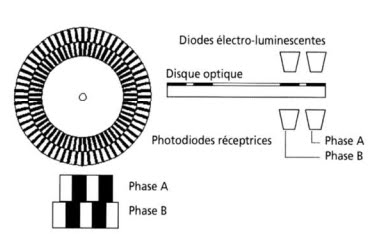
\includegraphics[width=0.5\textwidth]{images/codeurIncremental.jpg}
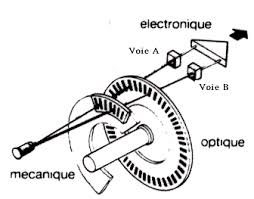
\includegraphics[width=0.5\textwidth]{images/schemaCodeurIncremental.jpeg}
\caption{Schema de codeurs incrémentaux}
\par\end{centering}
\end{figure}

\section{Caméra}
Il existe 2 types majoritaires de capteurs photographiques: CDD et CMOS. Cependant, un  nouveau type de capteur fait se popularise dans le milieu de la robotique: DVS.

\subsection{CDD}

\subsection{CMOS}

\subsection{DVS}
Un nouveau type de caméra fait son apparition: DVS (Dynamic Vision Sensor). Ce type de caméra n'enregistre pas une image à chaque pas de temps. Elle suit le même principe que les récepteurs lumineux dans nos yeux et enregistrement seulement les variations de luminosité. Ces caméras ont beaucoup de potentiel. En effet, puisque seulement la variation est enregistrée, il n'y a pas d'informations redondantes et les programmes peuvent être plus rapides. De plus, ces caméras sont plus aptes à enregistrer les mouvements rapides de part leur nature. Contrairement aux capteurs CDD et CMOS, il n'y a pas " de perte d'inforamtion" entre 2 images. Problème: les DVS coûtent très chères et ont encore une très faible résolution pour le prix demandé.

\subsection{Matériel}
\begin{description}
\item[Modèle:]
\item[Fabricant:]
\item[Fournisseur:]
\end{description}


\subsection{Utilisation}
\begin{description}
\item[Lecture de codes couleur:]
\item[Détection d'obstacle:]
\item[Positionnement d'objets sur le terrain:]
\end{description}

\chapter{Alimentation}

\section{Batterie}
Il existe 2 types majoritaires de batterie chimique. Les Lithium Polymère (LiPo) et les Nickel Mercure (Nimh).

\subsection{Lipo}
Ces batteries présentent la meilleure densité énergétique. Cependant, elles sont aussi très dangereuses. Elles peuvent en effet exploser et provoquer un feux chimique difficilement arrêtable.

Les choses suivantes peuvent causées l'explosion d'une LiPo.
\begin{itemize}
\item Mouillée
\item Percée
\item Recoit un choc
\item Laissée au soleil
\item Court-circuit
\end{itemize}

Si jamais la LiPo est bombée ou a des bosses, il faut absolument s'en débarasser. En attendant, la meilleure solution est de la placé dans un sceau en métal ou sur une surface non-inflammable (pierre, métal, ...). Ce type de batterie doit être jeté à la déchèterie dans la section réservée pour.

\subsection{Nimh}
Les batteries Nimh sont moins fragiles que les batteries Lipo. Cependant, elles ont une plus faible densité énergétique.

\subsection{Chargeur}
Les différents types de batterie ne se chargent pas de la même façon. Il y a un mode pour chaque sur le chargeur. Il faut aussi surveiller le taux de charge.

Pour les Lipo, il faut aussi brancher la prise d'équilibrage. Ce n'est pas obligatoire mais cela permet de prolonger la durée de vie de la batterie. En effet, au fur et à mesure des différents cycles de charge/décharge, les éléments de la Lipo ne vont pas avoir tous la même tension. La prise d'équilibrage permet d'empécher cela.


\section{Adapter l'alimentation}

\subsection{BEC}
Le BEC (Battery Eliminator Circuit) permet de délivrer une tension. Ce circuit appartient à l'électronique de puissance.

\subsection{Régulateurs de tension linéaire}
Les régulateurs permettent comme les BEC de fournir un

si pas de source de frais, dangereux

Inconvénients:
\begin{itemize}
\item Pas efficace, la tension a dissipé l'est sous la forme de chaleur
\item Cesse de d'alimenter en tension si la température dépasse un certain seuil
\end{itemize}

Avantages:
\begin{itemize}
\item Simple à mettre en oeuvre
\item Peu cher (de l'ordre de la dizaine de centimes)
\end{itemize}

\subsubsection{Utilisation}

Montage

\subsection{Convertisseur Buck}
C'est le type de circuit qui est utilisé dans 

Prix de l'ordre de l'euro

Utilise une bobine donc peut être source d'interférences électromagnétiques

\chapter{Composants électroniques}

\section{Fusible}

\subsection{PTC}

\subsection{Fusible réinitialisable}

\subsection{Thermistor}

\part{Programmation}

\chapter{Raspbian}

\section{Le Set up}
En règle général, il n'y aura pas d'écrans, de claviers ou de souris à disposition pour pouvoir utiliser directement la raspberry pi avec son ordinateur. Pour controurner ce problème, Matthieu Vignes(P14) a créé une configuration spéciale de l'image Raspbian.  Elle fait en sorte que dès le premier démarrage, la raspberry pi émet son propre réseau wifi sur lequel il est possible de se connecter pour pouvoir utiliser la raspberry pi.

La méthodologie pour créer cette image est disponible sur son Github:
\url{https://github.com/matthieuvigne/MiAM_eurobot2019/tree/master/ConfigRPi}

\begin{description}
\item[Windows:]Il faut installer Putty pour avoir accès au terminal de la raspberry pi. Sinon, il est possible d'avoir accès à la GUI avec VNC viewer.
\item[Linux:]Il faut utiliser les lignes de commandes.
\end{description}

\begin{description}
\item[sshfs:]Monter sur son système de fichier, un autre système de fichier distant, à travers une connexion SSH . En gros, il est possble d'avoir accès sur l'ordinateur à tous les fichiers de la raspberry pi. Les modifications sur l'ordinateur seront aussi réalisées sur la raspberry pi.
\item[ssh:]Créé une liaison SSH avec la raspberry pi, ce qui permet d'avoir accès à son terminal.
\item[scp:]Copie les fichiers de la raspberry pi à l'ordinateur et vice-versa par liaison SSH. 
\end{description}

Matériel utile:
\begin{description}
\item[Clef USB Wifi:]Permettra à l'ordinateur de se connecter à 2 réseaux Wifi en même temps: Celui de la raspberry pi et à une connection internet.
\item[Cable ethernet:]La raspberry Pi utilise déjà le wifi pour communiquer avec l'ordinateur. Il est alors nécessaire d'utiliser le cable ethernet pour pouvoir réaliser des mises-à-jours logiciel. Il faut pour cela faire un partage de connection par ethernet avec l'ordinateur.
\end{description}


\section{Le système d'exploitation}
Raspbian est un système d'exploitation basé sur Linux. Il est possible d'installer 2 versions sur la Raspberry Pi: la version lite (sans interface graphique), la version graphique (beaucoup plus lourde et gourmande en ressource). En règle générale, il es préférable d'installer la version Lite, cela laissera plus de puissance de calcul pour les programmes qui tourneront dessus.

\subsection{Les commandes utiles}
\begin{description}
\item[cd:]
\item[ls:]
\item[mkdir:]
\item[nano:]
\item[vim:]
\item[chmod:]
\item[apt install:]
\item[apt upgrade:]
\item[apt update:]
\end{description}

Pour lancer un programme binaire, il faut "./programme"

\subsection{Utiliser une clef USB}
Une clef USB ne peut pas être utilisé directement avec Linux, il faut la monter. Dans les OS avec interface graphique, cette étape se fait automatiquement mais pas si on utilise la verison Lite de Raspbian.

Trouver le périphérique:
lsblk

Le périphérique SUB apparaîtra dans le dossier /dev en général avec le nom sdb1. Il faut alors créer un dossier dans /media qui correspondra à notre clef USB.

sudo  mkdir /media/usb 

sudo mount /dev/sdb1 /media/usb

sudo umount /media/usb

\chapter{Le code}

Quel langage utilisé?

\section{Python}
Python, le langage que tout le monde maîtrise normalement après la prépa. Il est très facile de faire du prototypage avec. C'est d'ailleurs avec ce language qu'il faudra tester de nouvelles choses. Cependant, en tant que language interprété il est beaucoup plus lent que les languages compilés (C/C++).

\section{C/C++}

\subsection{Cross-compilation}
Il est possible de compiler les programmes en C et C++ sur la raspberry pi mais cela prends beaucoup de temps en raison du manque de puissance de calcul (de l'ordre des minutes). Cependant, une fois compiler une première fois, le compilateur ne devra recompiler que les fichiers modifiés. La compilation prendra alors moins de temps. 

En raison de l'architecture différente des processeurs sur l'ordinateur et sur la Raspberry Pi (ARM), il n'est pas possible de compiler les programmes sur l'ordinateur puis de les copier sur la Raspberry Pi. Il est cependant possible de simuler l'environnement de la raspberry pi pour la compilation sur ordinateur en utilisant la cross-compilation.

\chapter{Traitement de signaux GNSS: RTK Lib}

RTK Lib est un ensemble de programmes créés pour pouvoir exploiter et analyser les signaux obtenus à partir de récepteurs GNSS. Il existe un ensemble avec une interface graphique utilisable sous Windows. Il existe aussi une version UI utilisable sous n'importe quel système d'exploitation après avoir compiler les programmes en C.

Une branche a été créé à partir de RTK Lib: RTK Lib Explorer. Cette branch a été optimisée pour certains récepteurs et fonctionne en général mieux(en tout cas dans les cas vus).

\chapter{Traitement d'images: OpenCV}

OpenCV est la bibliothèque par excellence pour tout ce qui concerne le traitement d'images.

\section{Systèmes de couleur}
De part la manière dont nous voyons le monde, nous utilisons en général le système RGB pour décrire les couleurs. Cependant, ce n'est pas toujours le système de couleur le plus efficace pour étudier des images. En effet, certains éléments ressortiront plus dans un certain système de couleur. Par exemple, les feux de forêt sont plus distinct avec la luminescence du système LUV qu'avec le rouge de RGB.

\begin{figure}[h]
\begin{centering}
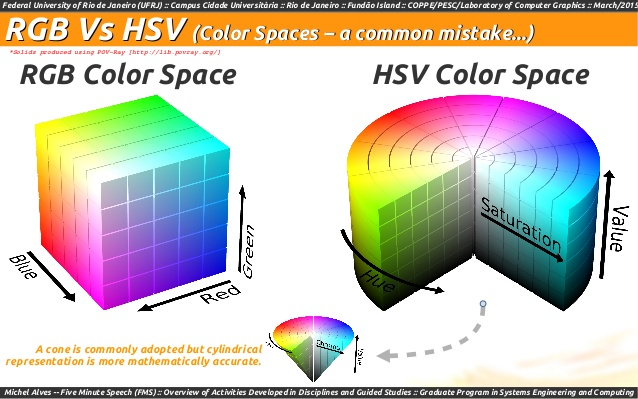
\includegraphics[width=0.7\textwidth]{images/RGB_HSV.jpg}
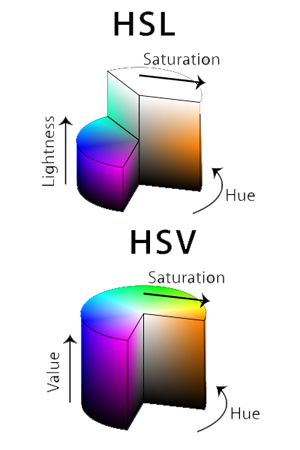
\includegraphics[width=0.7\textwidth]{images/HSL_HSV.jpg}
\caption{Systèmes de couleur}
\par\end{centering}
\end{figure}

\section{Odométrie visuel}

\url{https://link.springer.com/article/10.1186/s40064-016-3573-7}

\section{Vision stéréoscopique}
A partir de deux caméras dont on connaît la position relative, il est possible d'obtenir la profondeur de l'image. Cependant, cette méthode pour obtenir la profondeur est très sensible à différents paramètres tels que la calibration des caméras et la distance entre les caméras. Par ailleurs, la carte de profondeur générée est très approximative. Si on veut vraiment mesurer la profondeur d'une image, on utilisera plutôt une caméra infrarouge telle que la Kinect ou la Intel Realsense D435.

\begin{figure}[h]
\begin{centering}
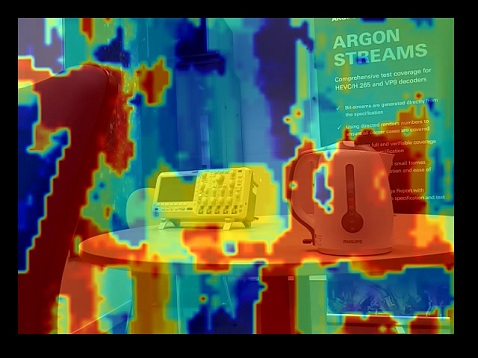
\includegraphics[width=0.6\textwidth]{images/depthMapStereo.jpg}
\caption{Profondeur d'image avec des stéréos caméras}
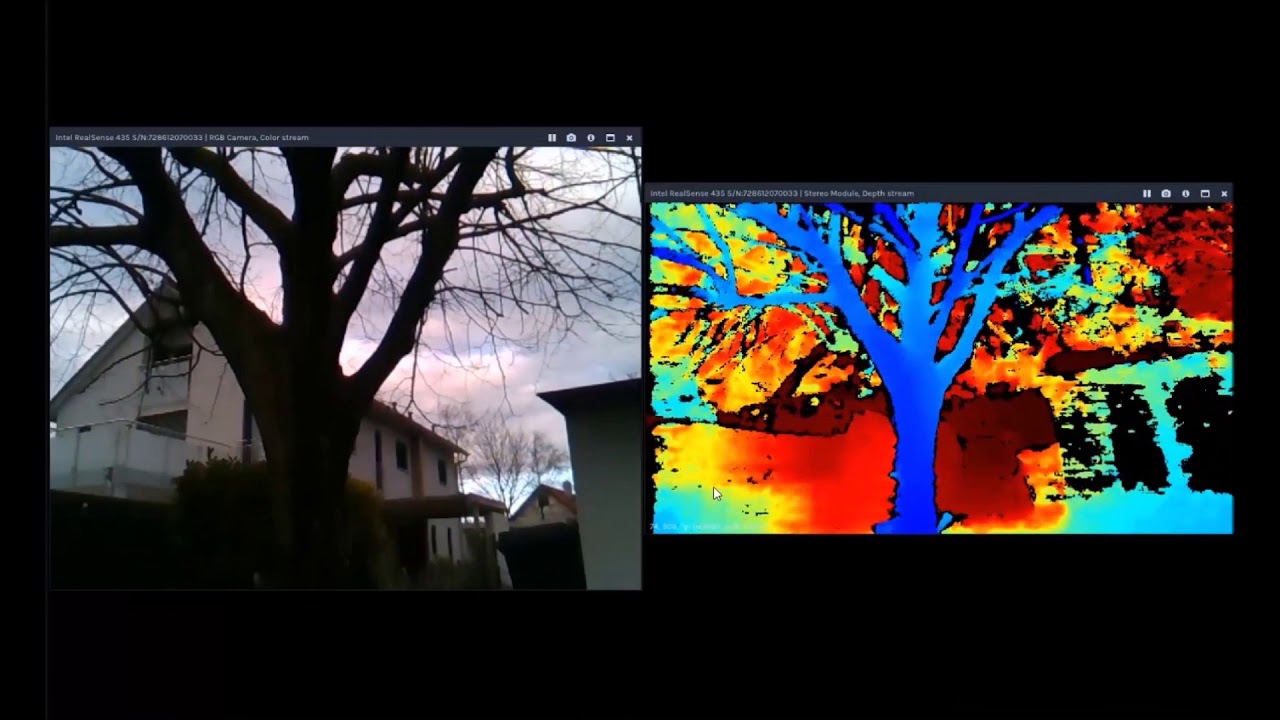
\includegraphics[width=0.6\textwidth]{images/depthMapRealSense.jpg}
\caption{Profondeur d'image avec RealSense D435 utilisant une caméra infrarouge}
\par\end{centering}
\end{figure}

\chapter{ROS}

ROS est une sorte de système d'exploitation pour la robotique.

Pourquoi l'utiliser:
\begin{itemize}
\item Une grande communauté
\item Beaucoup de bibliothèques déjà développées
\item Code beaucoup plus modulable
\item Possibilité de programmer un C/C++ ou en python (autres langages supportés aussi de manière non officielle)
\item Il est très souvent utilisé dans le milieu de la robotique
\end{itemize}

Cependant, ROS demande une certaine prise en main. Pour apprendre à l'utiliser, il a plusieurs solutions. Personnellement, je conseille ce livre disponible en version PDF\href{https://community.robotsource.org/t/download-the-ros-robot-programming-book-for-free/51}{"ROS Robot Programming Book"} . Il rassemble tout ce qui est nécessaire de savoir.

Cependant, pour avoir de la pratique, investir dans la plateform \href{https://www.robotigniteacademy.com/en/}{IgniteAcademy} est une très bonne idée. Un abonnement au mois coûte 39 euros. Je l'ai essayé et ça vaut vraiment le coût.

\chapter{Utilisation d'un Git}
Un Git est très pratique pour coder. Il permet travailler à plusieurs sur un même projet et surtout il permet de gérer l'évolution du code.

Il existe plusieurs services qui propose hébergements en ligne: Github, Gitlab,...  

\section{Méthodologie}

\begin{enumerate}
\item Avant de commencer, il faut récupérer la dernière version disponible du code.
\item Une fois satisfait avec les modifications réalisées sur un fichier, on enregistre la nouvelle version (vérifier que le code marche). Il faut mettre un commentaire au commit afin de garder une trace des modifiations réalisées.
\item Quand on a finit de travailler sur le code, on sauvegarde les modifications sur le serveur.
\end{enumerate}




\chapter{Protocole de communication}

Pour faire communiquer différents appareils électroniques entre eux, il existe plusieurs méthodes.

\section{Série}

\subsection{UART}

\subsection{TTL}

\section{I2C}

\section{SPI}

\section{CAN}
Ce protocole de communication a été développé par Bosch pour réduire la quantité de cable dans les voitures. Il permet en effet de faire communiquer plusieurs appareils avec seulement 2 fils.

\part{Automatique}

Le livre "Probabilistic Robotics" est excellent pour découvrir les différents problèmes de robotique. Il sert de très bonne introduction aux algorithmes de fusion de données pour estimer la position, au contrôle de robots et au SLAM.

\chapter{Estimation de l'attitude}

\section{Différentes manières de représenter l'attitude}

\subsection{Angles d'Euler}

\subsection{Vecteur rotation}

\subsection{Quaternion}

\section{Filtre complémentaire}

\section{Filtre de Mahony}

\section{Filtre de Madgwick}

\section{Filtre de Kalman}

\part{Machines de la menuiserie}

\chapter{Découpeuse Laser}

\chapter{Tour}

\chapter{Imprimante 3D}

\part{Conception}

\chapter{Général}

La règle d'or doit toujours être la SIMPLICITÉ. Il faut un système robuste et très répétable. Il y a toujours des imprévus (dimension de la table ou des objets à manipuler notamment).

\chapter{CAO}

\part{La Coupe de France de Robotique}

\chapter{Pendant l'année}
\begin{itemize}
\item Dès que du matériel est nécessaire, le commander immédiatement afin de l’avoir pour la semaine d’après. C’est souvent le matériel qui empêche de progresser sur les robots et de faire des test.
\end{itemize}
\chapter{Le départ}
\begin{itemize}
\item Faire une liste des outils et matières premières une semaine à l’avance afin de ne rien oublier. Il faudra cette liste à Mazouz.
\item Trouver un moyen pour déplacer les 2 robots et l’équipement nécessaire pour les préparer avec une seule personne. En effet, seulement 2 personnes peuvent aller jusqu’à la table de match et il peut être dur de tout porter à 2. Cela peut être un petit chariot comme le font d’autres équipes.
\end{itemize}

\chapter{La compétition}

\section{Les matchs}
\begin{itemize}
\item Faire une checklist de toutes les tâches à effectuer pour préparer le match. Avec le stress, il n’est pas rare d’oublier quelque chose et de faire rater le match.
\item Éviter vraiment de faire des changements de dernière minute. En 2017, RCV a perdu en demi-finale car ils ont choisi une stratégie non-testée. Un bug a empêché les 2 robots de démarrer.
\end{itemize}

\end{document}
